
%%%%%%%%%%%%%%%%%%%%%%%%%%%%%%%%%%%%%%%%%%%%%%%%%%%%%%%%%%%%%%%%%%%%%%%%%%%%%%%%
\section{Caracteristicas do som}

A música; na sua forma mais básica,  é um conjunto de sons; assim, 
a música é criada ao combinar sons, na justa medida, de 
ingênio, técnica e arte.

Entre as características de um som, temos \cite[pp. 12]{medteoria} :
\begin{description}
\item [Altura:] \label{sec:pos:Altura} 
Também chamado \textbf{tom}\footnote{A palavra tom tem vários significados em música, 
outro significado pode ser um intervalo ou distancia em frequência, 
utilizado na escala diatônica, para mais detalhes ir a Seção \ref{sec:notasmusicais}}, esta representa a frequência de vibração (principal) da onda mecânica que gera o sonido.
Isto é, que terão um altura maior os sonidos com maior frequência de vibração mecânica (mais agudos), 
e uma altura menor sonidos com menor frequência de brivação mecánica (mais graves).
\begin{example}
A campainha pra chamar ao atendente de um hotel, 
tem uma altura maior que a campana da igreja, 
que é tocada ao médio dia, que tem um sonido mais grave.
\end{example} 
\index{Música!Altura}\index{Música!Tom}
\item [Duração:] \label{sec:pos:Duracion}
Representa a longitude temporal, durante o qual um sonido será articulado.
\begin{example}
Podemos assoviar durante um tempo, curto, longo, muito longo, etc.
\end{example} 
\index{Música!Duração}
\item [Intensidade:] \label{sec:pos:Intensidade}
Se refere ao volume sonoro ou à potencia do sonido articulado, 
de modo que o som pode ter intensidades, por exemplo: fracas, fortes, muito fortes, etc.  
\begin{example}
Si escolhemos dois pedaços de madeira e batimos eles um contra outro, 
podemos gerar sons com diferente intensidade, dependendo da força com que realizemos os batimentos.
\end{example} 
\index{Música!Intensidade}
\item [Timbre:] \label{sec:pos:timbre}
Na definição da altura de um som, referenciamos esta seguindo a sua frequência principal,
porem um som não está composto exclusivamente por vibrações a esta frequência.
Na pratica os sons contem muitas outras frequências de vibração, que acontecem simultaneamente e 
que se manifestam com menor intensidade.
A combinação de todas estas frequências de vibração é o que gera o som que escutamos;
assim, a essa especifica configuração de frequências a chamamos como o timbre ou
a ``\textbf{cor}'' do som.
\begin{example}
Se geramos dois sons com a mesma altura; mas, um som articulado por uma flauta,
e o outro por um violão, ambos sons terão diferentes timbres ou cores.
\end{example} 
\index{Música!Timbre}
\end{description}
~\\

%%%%%%%%%%%%%%%%%%%%%%%%%%%%%%%%%%%%%%%%%%%%%%%%%%%%%%%%%%%%%%%%%%%%%%%%%%%%%%%%
\section{Elementos da música}
Conhecidas estas definições básicas, e procurando estruturas mais complexas na música,
podemos distinguir alguns elementos com que esta é constituída \cite[pp. 11]{alves2004teoria}, 
por exemplo temos:

\begin{description}
\item [Ritmo:] \label{sec:pos:Ritmo}
Se refere a distribuição temporal da execução dos sons e a proporção na duração destes. 
Asim, o ritmo carateriza à música no âmbito temporal \cite[pp. 11]{medteoria}.
\index{Música!Ritmo}
\begin{example}
Batendo palmas, criamos a sequencia de sons: palmas, pausa curta, palmas, palmas, pausa loga e palmas.
\end{example} 
\item [Melodia:] \label{sec:pos:Melodia}
É um conjunto de sons, que podem ter diferentes \hyperref[sec:pos:Altura]{\textbf{alturas}}, 
e que estão dispostos sequencialmente. 
A melodia representa um elemento horizontal\footnote{\label{eixohor}Eixo horizontal: Eixo com múltiplas distribuições de tempo dos sons na música} na música, ver Figura \ref{fig:melodia},
e esta é indivisível do ritmo \cite[pp. 517]{apel1969harvard} \cite[pp. 11]{medteoria}.
\begin{example}
Se assoviamos ``parabéns pra você'', estamos executando uma melodia 
(executando diferentes sons numa distribuição temporal específica).
\end{example} 
\index{Música!Melodia} 
\item [Harmonia:] \label{sec:pos:Harmonia}
Conjunto de sons dispostos simultaneamente em \hyperref[sec:pos:Altura]{\textbf{alturas}} diferentes.
A harmonia representa um elemento vertical\footnote{\label{eixover}Eixo vertical: Eixo com múltiplas distribuições de frequência dos sons na música} na música \cite[pp. 371]{apel1969harvard} \cite[pp. 8]{cardoso1973curso} \cite[pp. 11]{medteoria}, 
ver Figura \ref{fig:harmonia}. 
\begin{example}
Se num piano pressionamos simultaneamente as teclas: Do, Mi e Sol. Estamos executando uma harmonia.
\end{example} 
\index{Música!Harmonia} 
\item [Contraponto:] \label{sec:pos:Contraponto}
O termo deriva de ``punctus contra punctum'' que significa ``nota contra nota'', 
e por extensão ``melodia contra melodia''. 
Assim, falar de contraponto é equivalente a dizer, dois ou mais melodias executadas simultaneamente  
(concepção horizontal\footref{eixohor} e vertical\footref{eixover} da música)  \cite[pp. 208]{apel1969harvard} \cite[pp. 11]{medteoria}.
\begin{example}
Uma orquestra com vários músicos tocando cada um uma melodia.
\end{example} 
\index{Música!Contraponto}
\end{description}


\begin{figure}
    \centering
    \begin{subfigure}[b]{0.75\textwidth}
        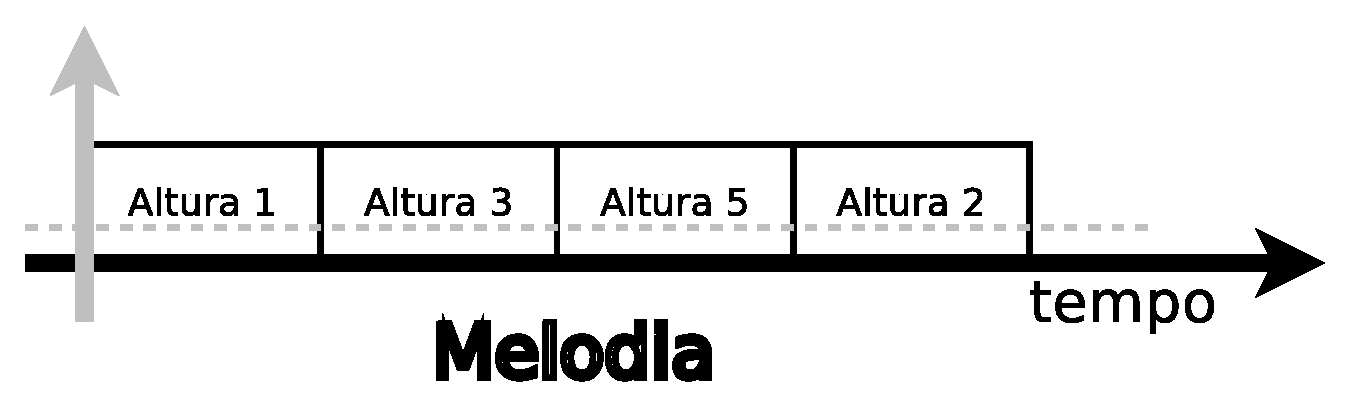
\includegraphics[width=\textwidth]{chapters/cap-musica-basica/melodia}
        \caption{Melodia representada no eixo horizontal.}
        \label{fig:melodia}
    \end{subfigure}
    ~ %add desired spacing between images, e. g. ~, \quad, \qquad, \hfill etc. 
      %(or a blank line to force the subfigure onto a new line)
    \begin{subfigure}[b]{0.75\textwidth}
        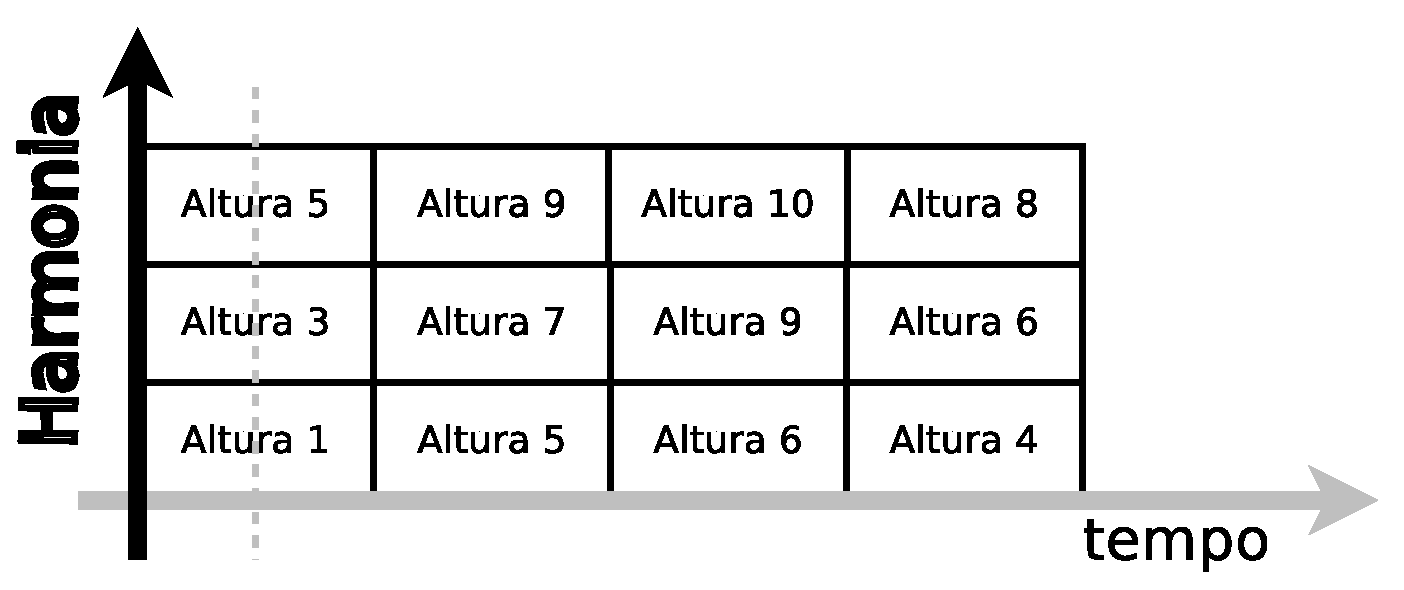
\includegraphics[width=\textwidth]{chapters/cap-musica-basica/harmonia}
        \caption{Harmonia representada no eixo vertical.}
        \label{fig:harmonia}
    \end{subfigure}
    \caption{Eixo horizontal e vertical na música.}\label{fig:meloharmo}
\end{figure}


